\section{Distributed Acoustic Sensing}
\label{back:das}

\acrfull{das} is a type of sensing where one use fiber optic cables to measure strain sensing. By using a optoelectronic device such as a OptoDAS, frequency strains can be measured over vast distances. They are heavily used for monitoring conditions within geophysical environments, such as movement of traffic, land slides, maritime wildlife and much more. Due to their high sensitivity, measuring irregularities is and analyzing this is a very common task. 

\begin{figure}[!h]
    \centering
    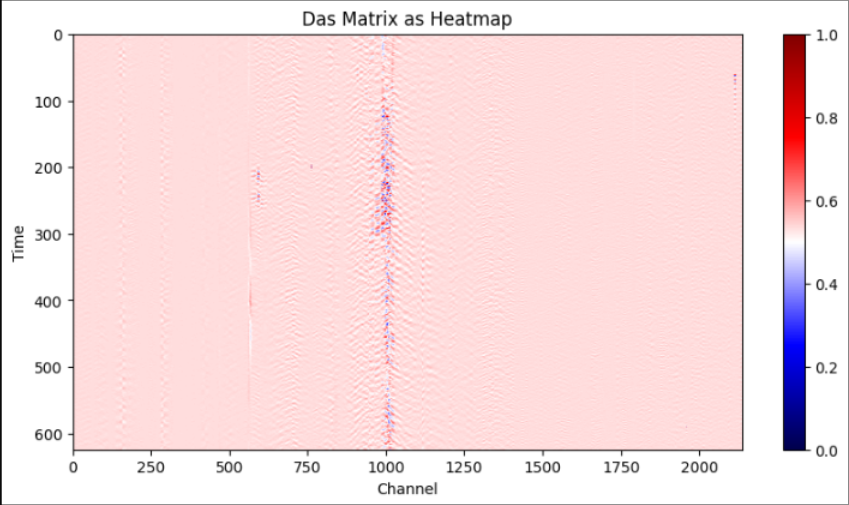
\includegraphics[width=0.7\linewidth]{figures/das_example.png}
    \caption{DAS data frame example}
    \label{fig:dasframe-ex}
\end{figure}

\subsection{Numerical analysis}

When \acrshort{das} data is recorded, it can be stored in several different file formats. Data stored in \acrshort{hdf5} files have the advantage of storing additional metadata beside it, but memory mapped matrix files works if the data doesn't depend on too much pre processing. Timestamps, channel decimation, strain, gauge length and sample rate are the most crucial ones to be able to handle this data. 

\textbf{Timestamp} is the stored time of the first recording in the file.

\textbf{Gauge length} is the distance between each sensor that stores this data.

\textbf{Channel decimation} explains which channels are stored. Not all channels along the total measurement is stored, and so to understand the location of a signal, the gauge length in combination with the channel decimation tells us the exact distance from the start of the measurement.

\textbf{Sample Rate} is measured in hertz, and explains the amount of recordings per second.

Then there is the data itself, which is stored in a matrix format as shown in table \ref{tab:das}.

\begin{table}[h]
\centering
\begin{equation*}
\mathbf{X} = \begin{bmatrix}
x_{1,1} & x_{1,2} & \cdots & x_{1,n-1} & x_{1,n} \\
x_{2,1} & x_{2,2} & \cdots & x_{2,n-1} & x_{2,n} \\
\vdots & \vdots & \ddots & \vdots & \vdots \\
x_{t-1,1} & x_{t-1,2} & \cdots & x_{t-1,n-1} & x_{t-1,n} \\
x_{t,1} & x_{t,2} & \cdots & x_{t,n-1} & x_{t,n}
\end{bmatrix}
\end{equation*}
\caption{Matrix representation of DAS data with $n$ channels and $t$ timestamps}
\label{fig:dasmatrix}
\end{table}


In the matric $A$ above, $t$ denotes the max amount of recordings for the file; for one second this would be equal to the sample rate. $c$ is the max index of channels. In this way, channels are stored column-wise, and samples row-wise. Depending on whats more interesting to analyze, this matrix may be transposed to speed up calculations.